\chapter{Einleitung}

Die Einleitung gibt einen Überblick über die Entstehung und die Zielsetzung dieser Bachelorarbeit. Sie skizziert den Hintergrund der Zusammenarbeit mit der Abteilung CSC FI OES LMS der Infineon Technologies AG und erläutert die Motivation für die Entwicklung eines automatisierten technischen Feasibility Checks. Darüber hinaus wird der methodische Ansatz zur Umsetzung der Lösung vorgestellt sowie die Struktur der Arbeit näher beleuchtet. Dieser Abschnitt bildet den Ausgangspunkt, um die nachfolgenden Kapitel systematisch zu erschließen und einen klaren Rahmen dafür zu schaffen.

\section{Motivation}
Die Idee der vorliegenden Arbeit entstand in Zusammenarbeit mit der Abteilung CSC (Corporate Supply Chain) FI (Factory Integration) OES (Optimization \& Execution Solutions) LMS (Lab Management Solutions) der Infineon Technologies AG. 
In der Abteilung arbeite ich schon seit circa zwei Jahren als Werkstudent an Themen wie Web- und Mobile-App-Entwicklung unter meinen zwei Betreuern Florian Saller und Fabian Vilsmeier.
Zusammen mit diesen und Thomas Gombocz, der bei Infineon in München beschäftigt ist, habe ich mein Thema des ''automatisierten technischen Feasibility Checks für die Durchführung von Qualifikationen neuer Halbleiter-Produkte'' ausgearbeitet.

\section{Zielsetzung der Arbeit}
In dieser Bachelorarbeit wird ein sogenannter automatisierter technischer Feasibility Check, zu deutsch Machbarkeitsstudie, geplant und umgesetzt. Dieser ist Bestandteil einer größeren internen Software-Applikation namens \gls{REALIS}, welches
im Zuge einer Migration von einer Windows-Applikation zu einer Web-Applikation zusätzlich verbessert und modernisiert werden soll. Dabei ist der Feasibility Check ein Feature, dass zuvor manuell von Anwendern durchgeführt werden musste, und nun automatisiert werden soll.

Der technische Feasibility Check soll nahtlos in das System \gls{REALIS} integriert werden. Dabei wird er als Backend-Logik in der Programmiersprache C\# umgesetzt. Diese Logik kann durch einen einfachen Aufruf vom Frontend aus gestartet werden, wobei der Algorithmus auf Daten in der Datenbank zugreift und dem Anwender anschließend ein Ergebnis zur Verfügung stellt.

Neben der Backend-Entwicklung werden in dieser Arbeit auch ein erweitertes Datenbankmodell konzipiert, um bestimmte Einstellungen und Ergebnisse des Feasibility Checks zu speichern, und zwei verschiedene Frontends mit Angular, für die Web- bzw. native App Darstellung, ausgearbeitet \todo{was noch alles?}.

\section{Software-Entwicklungsprozess}
Software-Entwicklungsprozesse werden durch sogenannte Vorgehensmodelle strukturiert. Diese Modelle dienen dazu, die Organisation von Software-Entwicklungs\-projekten zu unterstützen, indem sie sämtliche Aktivitäten systematisch in klar definierte und verbindliche Arbeitsschritte gliedern.

Für dieses Projekt wird das Prototyping-Modell eingesetzt. In diesem Ansatz werden schrittweise Prototypen basierend auf den aktuellen Anforderungen entwickelt. Das daraufhin eingeholte Feedback von Auftraggebern oder Endanwendern ermöglicht eine kontinuierliche Verfeinerung der Anforderungen und eine schrittweise Verbesserung des Prototyps. Die Stadien dieses Modells werden in Abbildung~\ref{fig:Prototyping-Modell} nochmals verdeutlicht \cite{senarath2021waterfall}.

\begin{figure}[h!]
    \centering
    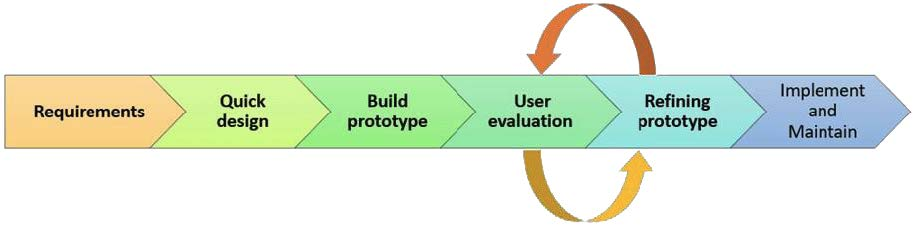
\includegraphics[]{bilder/Prototyping_Stages.jpg}
    \caption{Prototyping-Modell Stadien \cite{senarath2021waterfall}}
    \label{fig:Prototyping-Modell}
\end{figure}


Das Prototyping-Modell wurde eingesetzt, da die Anforderungen des technischen Feasibility Checks zu Beginn noch nicht eindeutig definiert waren und erst im Laufe der Entwicklung bestimmte Aspekte geklärt werden konnten. Außerdem wird das Risiko von Fehl-Entwicklungen minimiert, da der Anwender Ergebnisse schneller evaluieren kann. Zudem fördert dieses Vorgehen den regelmäßigen Austausch zwischen dem Entwickler und den Auftraggebern \cite{senarath2021waterfall}.

\section{Aufbau der Arbeit}
Die Bachelorarbeit ist so strukturiert, dass nach diesem einleitenden Kapitel in Abschnitt \ref{Chap:TheoretischeGrundlagen} die wichtigsten theoretischen Grundlagen erklärt werden. 
Hierbei wird kurz das Unternehmen Infineon Technologies AG vorgestellt und anschließend die Halbleitertechnologie behandelt. Danach wird auf die Software-Applikation \gls{REALIS} eingegangen und der technische Feasibility Check erläutert.

Im nächsten Schritt werden im Kapitel \textit{\nameref{Chap:Anforderungen}} die technischen und funktionalen Anforderungen beschrieben, die durch das Prototyping-Modell schrittweise verbessert und bei Bedarf erweitert worden sind. Zusätzlich wird eine Stakeholderanalyse durchgeführt.

Zur Realisierung der Lösung wird ein Design erstellt, das dann im Kapitel \textit{\nameref{Chap:Implementierung}} umgesetzt wird. Das Kapitel Test beschreibt die Testmethodik. Abschließend werden die während der Arbeit aufgetretenen Herausforderungen reflektiert und ein Fazit gezogen. Darüber hinaus wird ein Ausblick auf potenzielle Optimierungen und Erweiterungen des Systems bzw. Algorithmus gegeben.





